\section{Code Generator}
\subsection{Aufgabe}
\textbf{Erzeugung von ausführbarem Maschinencode}
\begin{itemize}
    \item Input: Zwischendarstellung (Symboltabelle + AST)
    \item Output: Maschinencode
\end{itemize}
\textbf{Mögliche Zielmaschinen}
\begin{itemize}
    \item Reale Maschine, z.B. intel 64, ARM Prozessor
    \item VM, z.B. JVM, .NET CLI
\end{itemize}

\subsection{Unsere Zielmaschine}
\textbf{Kernkonzepte}
\begin{itemize}
    \item Virtueller Stack-Prozessor: keine Register
    \item Branch Instructions (Goto): Programmfluss steuern
    \item Metadaten
\end{itemize}

\subsection{Stack Prozessor}
\begin{itemize}
    \item Instruktionen benutzen Auswertungs-Stack
    \item Keine Register wie auf echten Prozessoren
\end{itemize}

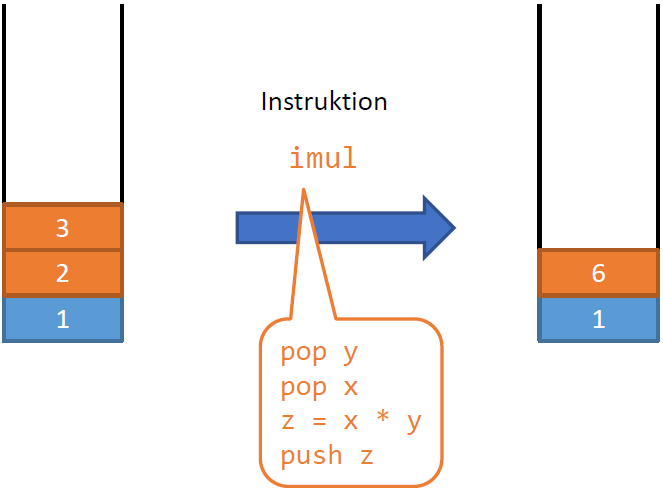
\includegraphics[width=0.5\linewidth]{stack_prozessor.png}

\subsection{Auswertungs-Stack}
\begin{itemize}
    \item Jede Instruktion hat definierte Anzahl von Pop- und Push-Aufrufen
    \item Eigener Stack pro Methodenaufruf
    \item Stack hat unbeschränkte Kapazität
\end{itemize}
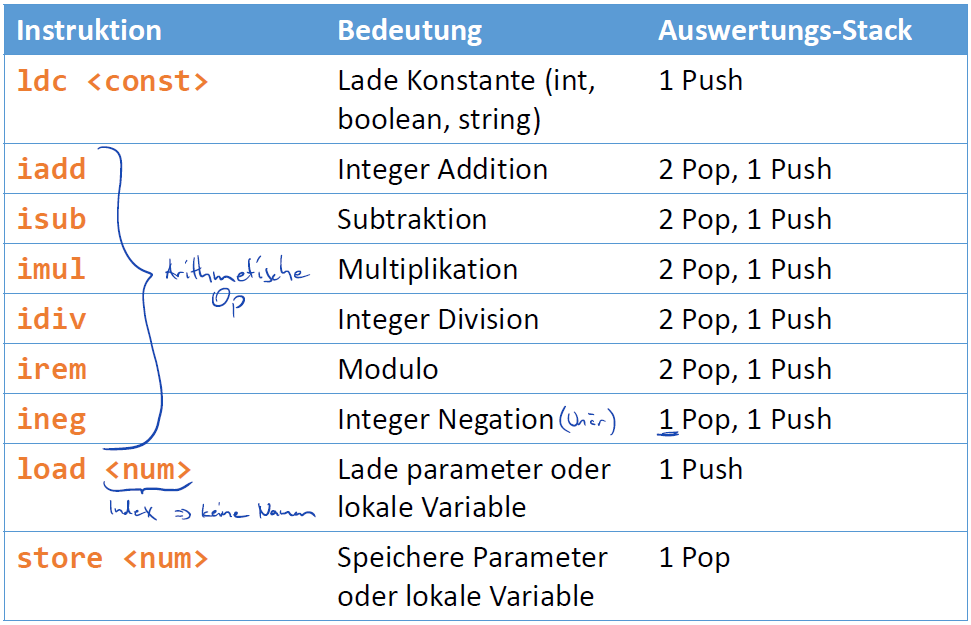
\includegraphics[width=0.5\linewidth]{instruktionen.png}

\subsubsection{Load/Store Nummerierungen}
\begin{itemize}
    \item \textit{this} Referenz: Index 0
    \item Danach, $n$ \textbf{Parameters}: Index $1..n$
    \item Danach, $m$ \textbf{lokale Variablen}: Index $n+1...n+m$
\end{itemize}
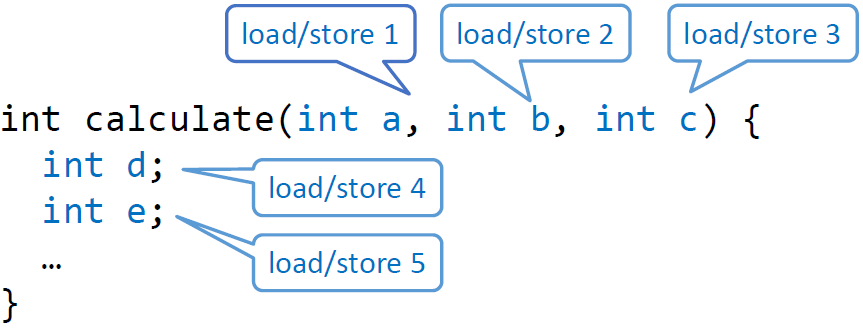
\includegraphics[width=0.5\linewidth]{load_store.png}

\subsubsection{Compare-Instruktionen}
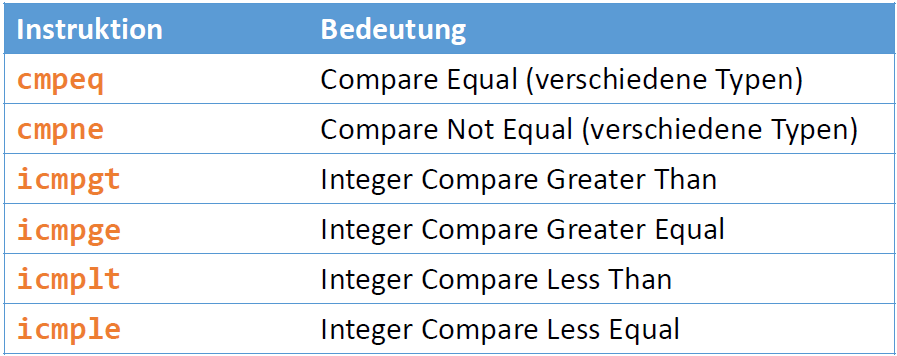
\includegraphics[width=0.5\linewidth]{compre_instruktionen.png}\\
\textbf{Pop right, Pop left, Push boolean}

\subsubsection{Branch-Instruktionen}
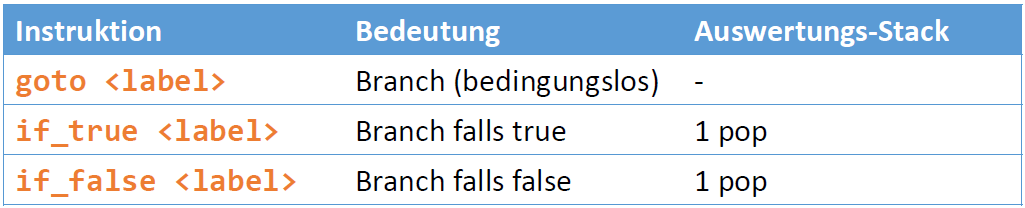
\includegraphics[width=0.5\linewidth]{branch_instruktionen.png}\\

\subsubsection{Metadaten}
\begin{itemize}
    \item Zwischensprache kennt alle Informationen zu
    \begin{itemize}
        \item Klassen (Namen, Typen der Fields und Methoden)
        \item Methoden (Namen, Parametertypen und Rückgabetyp)
        \item Lokale Variablen (Typen)
    \end{itemize}
    \item Kein direktes Speicherlayout festgelegt
    \item Nicht enthalten
    \begin{itemize}
        \item Namen von lokalen Variablen und Parameter
        \item Diese sind nur nummeriert
    \end{itemize}
\end{itemize}
\textbf{Verwendung:}
\begin{itemize}
    \item Speicherplatz-Allozierung
    \item Fehlermeldungen
    \item Funktionsaufrufe
\end{itemize}

\subsection{Code Generierung}
\begin{enumerate}
    \item Traversiere Symboltabelle: Erzeuge Bytecode Metadaten
    \item Traversiere AST pro Methode (Visitor): Erzeuge Instruktionen via Bytecode Assembler
    \item Serialisiere in Output Format
\end{enumerate}

\subsubsection{Backpatching}
\begin{itemize}
    \item Branch Offsets auflösen
    \item Label: relativer Instruktions-Offset ab Ende der aktuellen Branch-Instruktion
\end{itemize}

\subsubsection{Template-Basierte Generierung}
\begin{itemize}
    \item Postorder-Traversierung: Kinder zuerst besuchen
    \item Jeweils Template für erkanntes Teilbaum-Muster anwenden
\end{itemize}

\subsubsection{Short-Circuit Semantik}
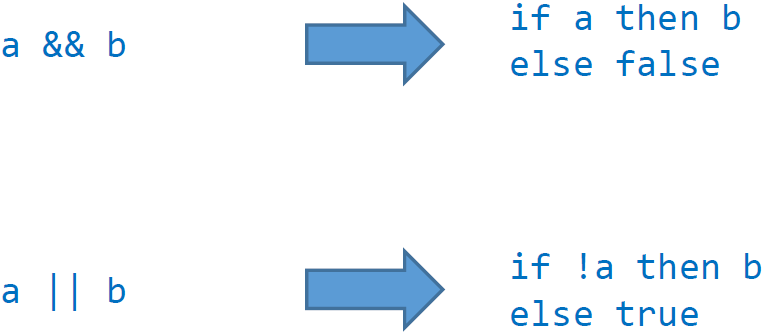
\includegraphics[width=0.5\linewidth]{short_circuit.png}

\subsubsection{Methodenaufruf}
\textbf{Statisch}
\begin{itemize}
    \item Vordefinierte Methoden: $readInt()$ etc.
\end{itemize}
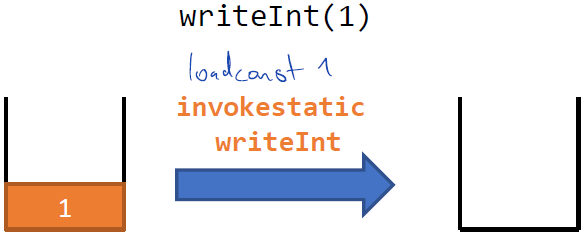
\includegraphics[width=0.4\linewidth]{static1.png}
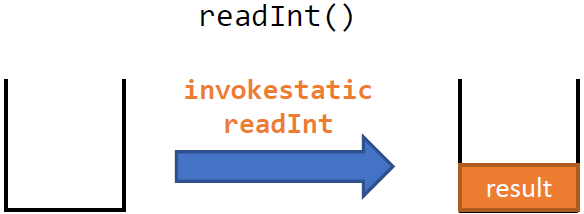
\includegraphics[width=0.4\linewidth]{static2.png}
\vspace{1cm}\\

\textbf{Virtuell}
\begin{itemize}
    \item Alle anderen Methoden
\end{itemize}
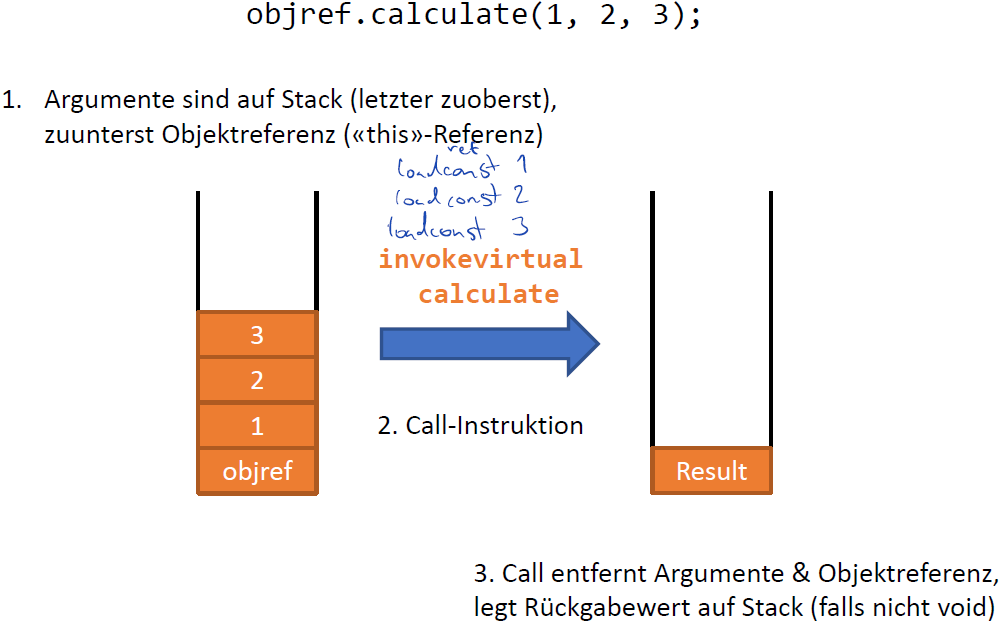
\includegraphics[width=0.5\linewidth]{virt.png}

\subsubsection{Parameter \& Rückgabe}
\begin{lstlisting}
int sum(int x, int y) {
    return x + y;
}

load 1 // load param x
load 2 // load param y
iadd // x + y
ret // return from method (auch bei void, max 1 Wert auf Stack)
\end{lstlisting}